\documentclass[10pt,journal,compsoc]{IEEEtran}
\title{Basketball movement tracking}
\author{\IEEEauthorblockN{Wei Hong (\it wh951\rm)}\\
\and\IEEEauthorblockN{Nan Wang (\it nw953\rm)}\\\ \\\and{CS-GY6083 Computer Vision} \\\and{May 2016}}

\usepackage{amsmath}
\usepackage{amsfonts}
\usepackage{amssymb}
\usepackage{courier}
\usepackage{algorithmic}
\usepackage{graphicx}
\usepackage{subfig}

\begin{document}
\maketitle
\section{\textbf{introduction}}
\IEEEPARstart{s}{hooting} is the most important scoring technique in a basketball match. Professional and amateur players are always eagle to improve their shooting skills. However, it is difficult to analyze a shoot and get its trace by raw eyes. So we would like to develop a system which can help people get the 3D basketball trace from the video and is easy to easy.
\section{\textbf{Approach}}
\subsection{System Setup}
The idea is to reconstruct the ball movement curve when shooting the basketball. We want to do the reconstruction by calculating the world coordinates of the basketball in each frame of the video. 
\\For the system we developed, it only needs two smart phones with tripods. The location, distance and angle of the smart phone are arbitrary as long as the basketball is within the scenes and we did not calibrate them before we shot the videos. We thought it would be difficult or impossible for the users to measure these parameters and calibrate in practical use since it would need extra tools such as rule, semicircular instrument, etc. and take at least dozens of minutes.
\begin{figure}[h]
\centering
%\subfloat[][setup]
{
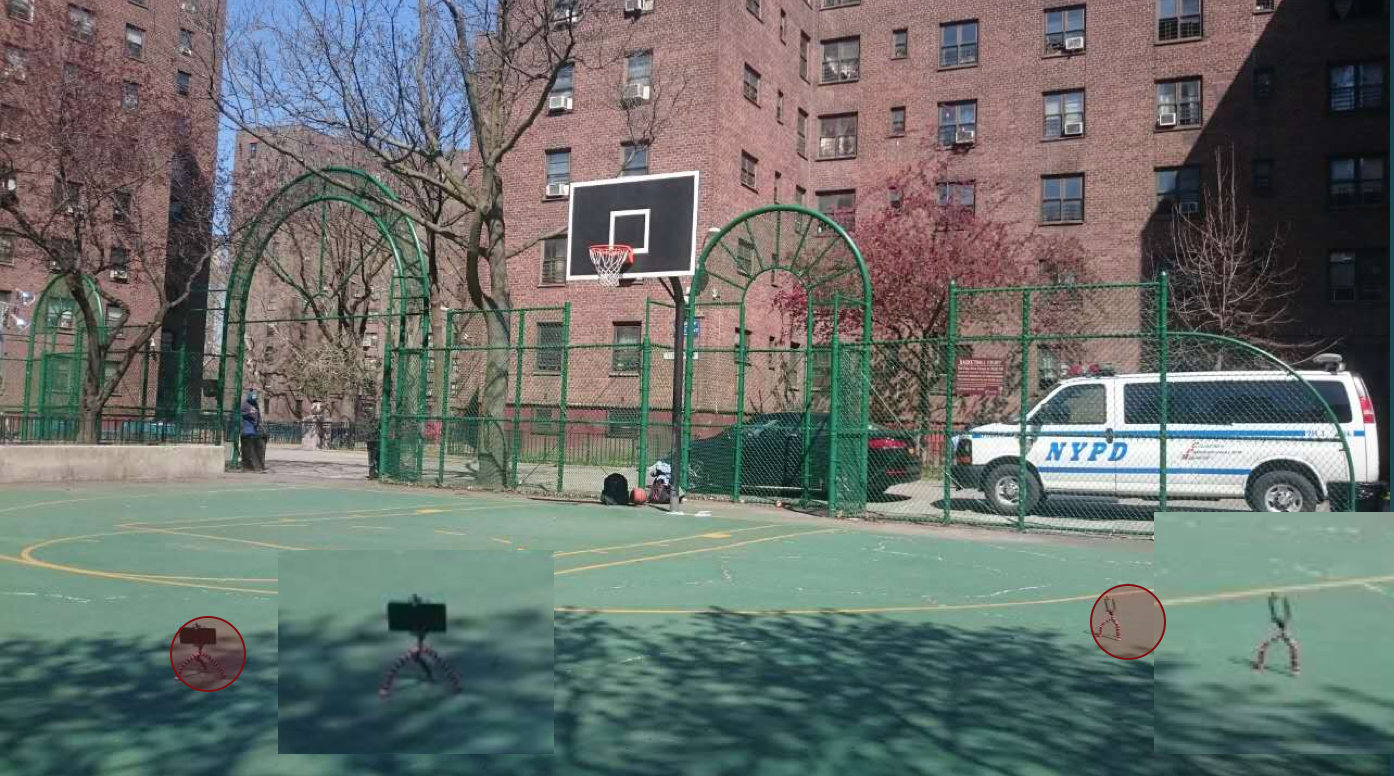
\includegraphics[width=3.4 in]{setup.png}
}
\caption{two smart phones with tripods}
\end{figure}
\subsection{Data collection}
After we have captured two videos, we use matlab to extract every frame pictures of videos and choose the useful cosponding frame.
\begin{figure}[h]
\centering
\subfloat[][first camera]
{
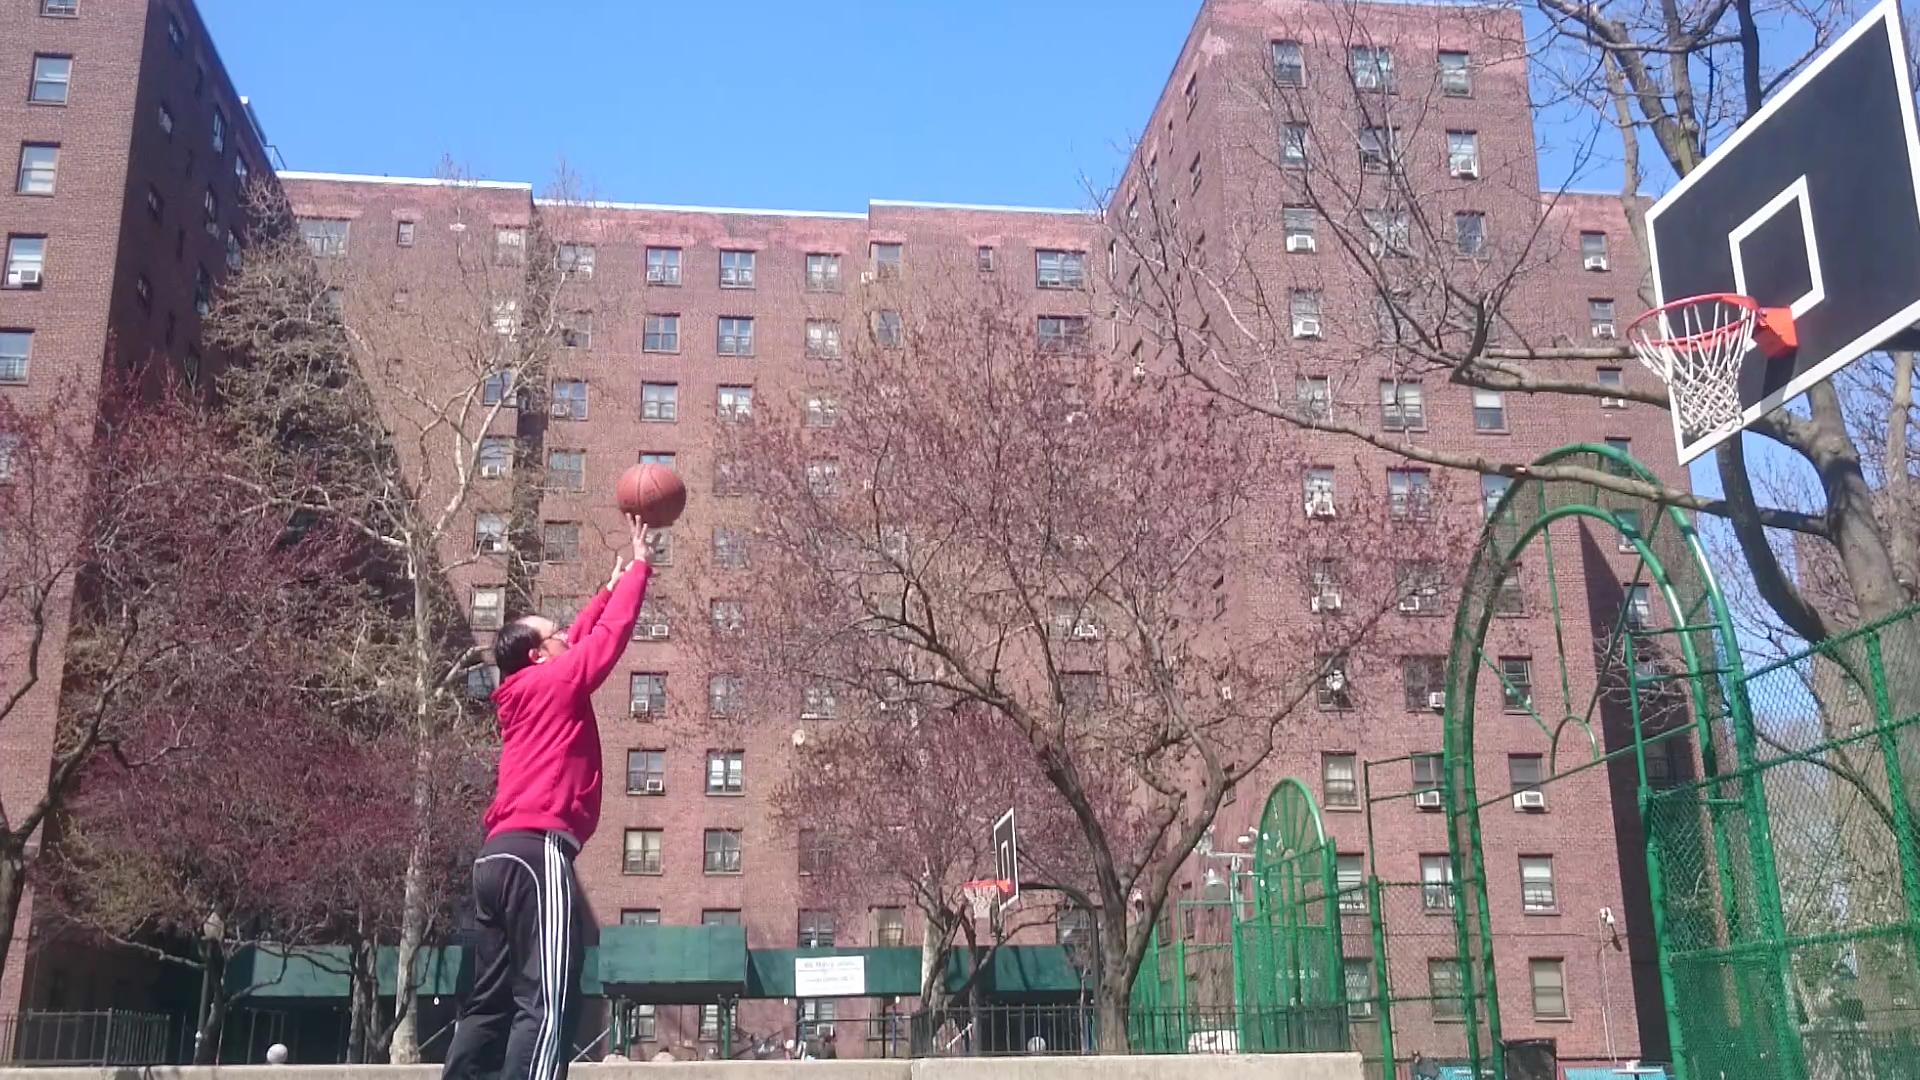
\includegraphics[width=1.6 in]{nan0.jpg}
}
\subfloat[][second camera]
{
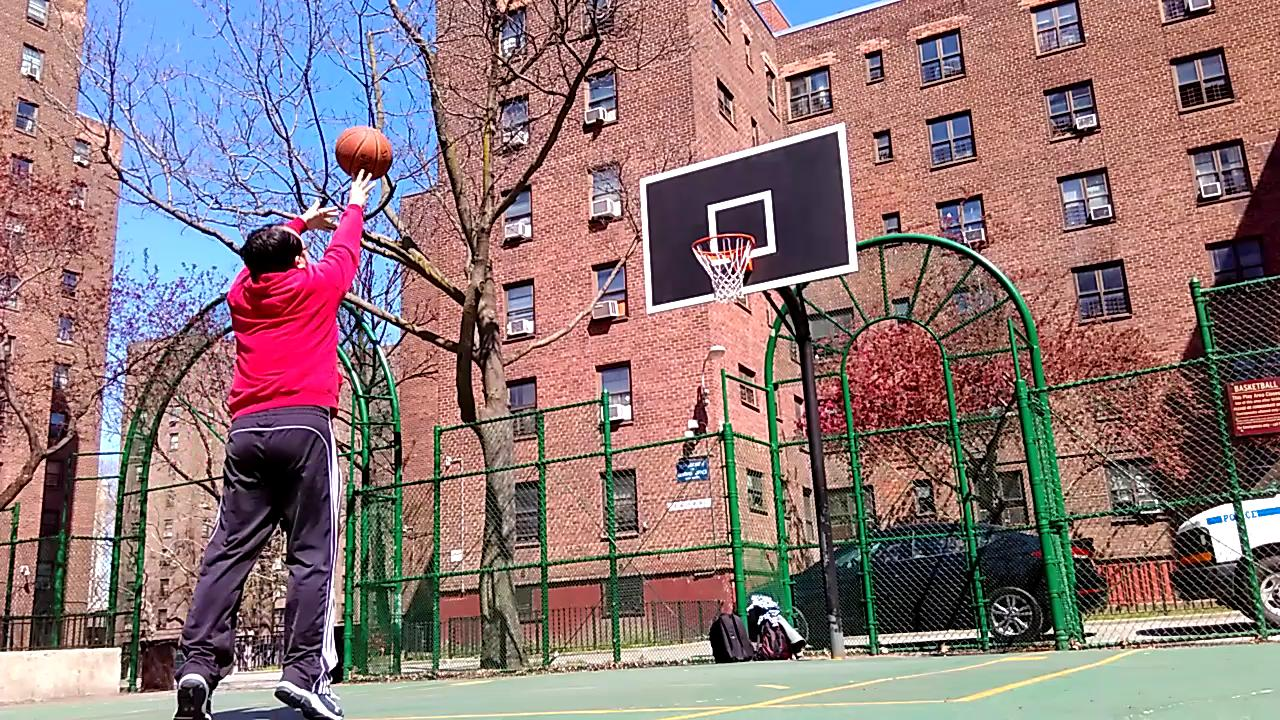
\includegraphics[width=1.6 in]{wei0.jpg}
}
\caption{first frames of shooting of two cameras}
\end{figure}
\\Next step is to pick up the center of ball in each frame. According to the geometry of perspective, whenever a ball is viewed, it is always a circle at any angle, and the center of a ball is also the center of a circle. Then center points of basketball in the frames manually can be got by picking up the center of the basketball.
\begin{figure}[h]
\centering
\subfloat
{
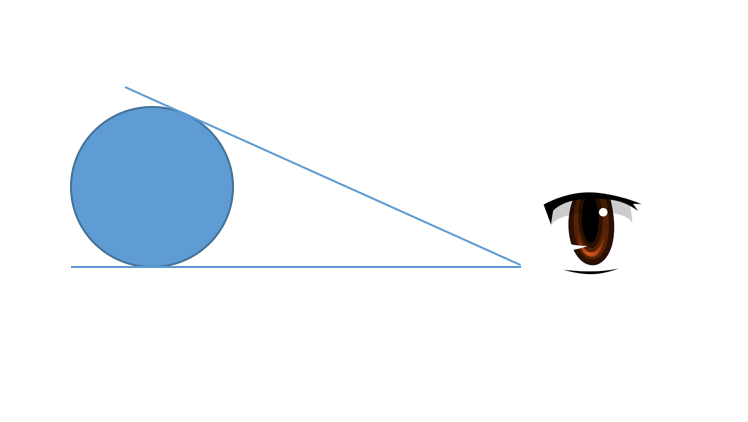
\includegraphics[width=3.4 in]{ball_view.png}
}
\caption{Perspective of a ball}
\end{figure}

\begin{figure}[h]
\subfloat
{
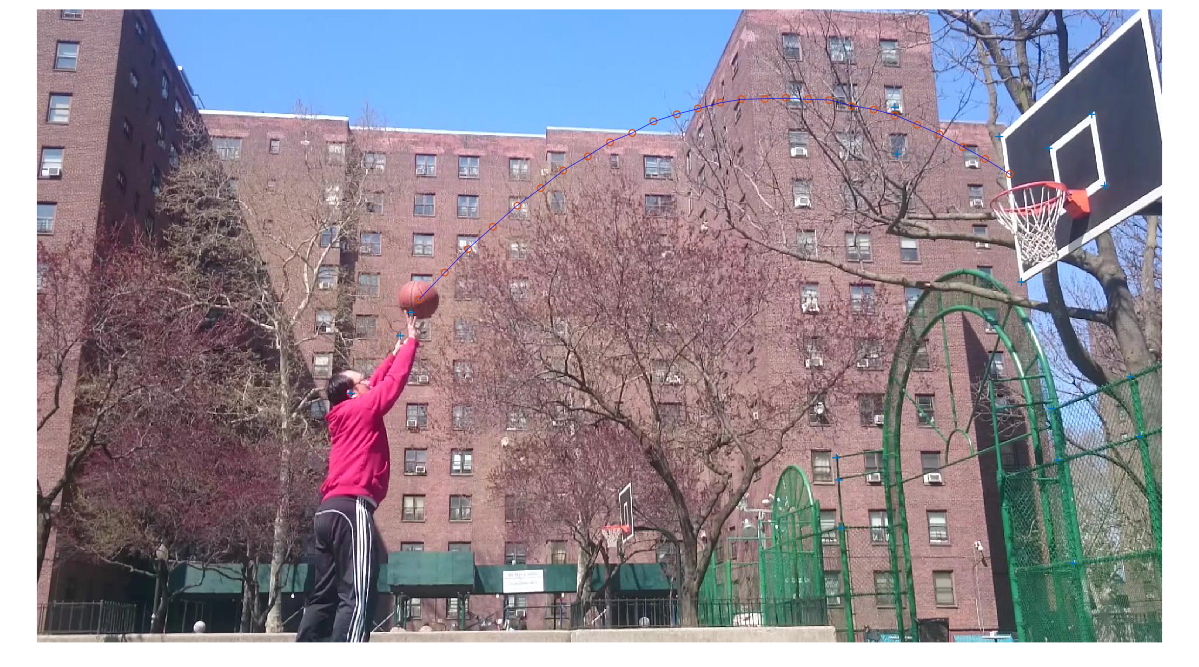
\includegraphics[width=3.4 in]{balltrace_nan.png}
}
\caption{Trace of the basketball in the first camera}
\end{figure}

\begin{figure}[h]
\subfloat
{
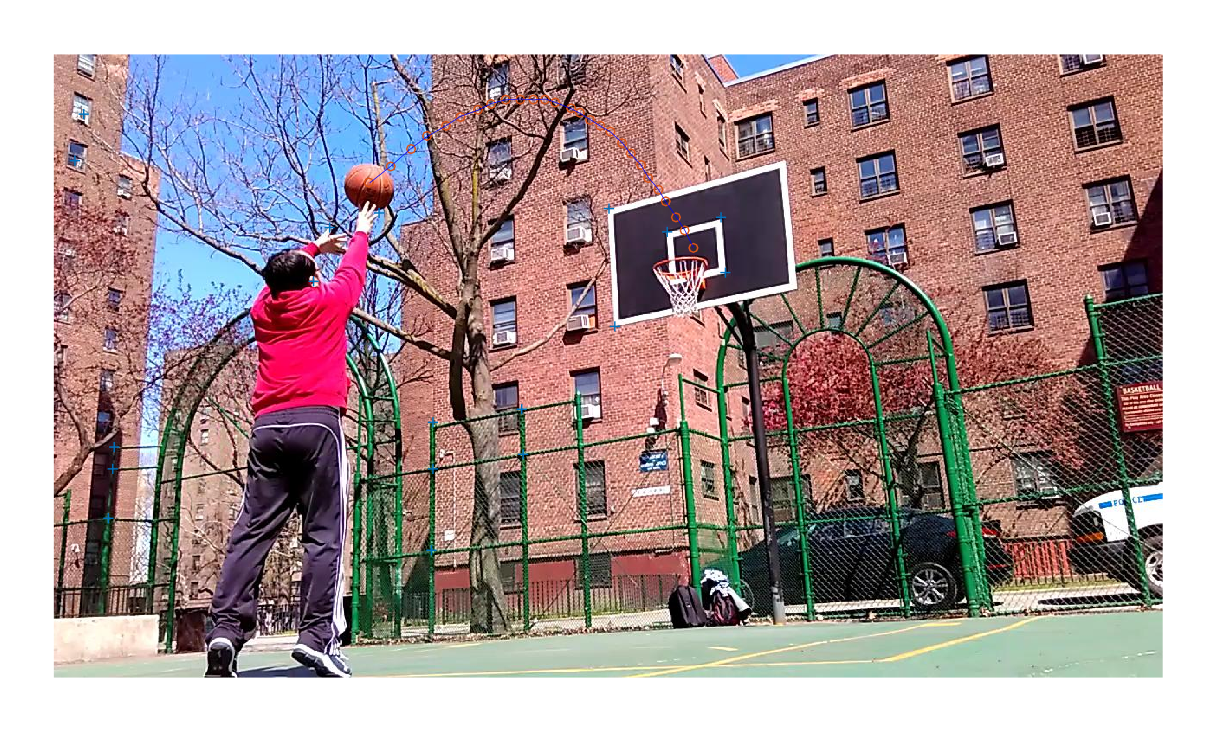
\includegraphics[width=3.4 in]{balltrace_wei.png}
}
\caption{Trace of the basketball in the second camera}
\end{figure}

\section{\textbf{algorithms}}
\subsection{camera calibration}
First, the intrinsic matrices $K$ and $K'$ are required in our future calculations. We can obtain the intrinsic parameters
of the cameras through camera calibration, and thus the matrices can be calculated.\\
The calibration has been performed on both of the cameras.\\
\begin{figure}[h]
\centering
%\includegraphics[width=2.5in]{cali_nan.jpg}
\caption{camera calibration}
\end{figure}

\subsection{calculate the fundamental matrix and essential matrix}
The second step is to calculate the fundamental matrix between the two cameras. By selecting corresponding point pairs $u$ 
and $u'$ on videos taken by the two cameras, the fundamental matrix can be calculated by establishing equations of the form
 $u^{T}Fu'=0$. \\
 We have chosen more than 8 points, so the equations are a over constrained system. In this case, the 
 fundamental matrix is calculated by minimizing the least square error.\\
\begin{figure}[h]
\centering
\subfloat[][first camera]
{
%\includegraphics[width=1.2in]{funmat_nan.jpg}
}
\subfloat[][second camera]
{
%\includegraphics[width=1.2in]{funmat_wei.jpg}
}
\caption{calculating fundamental matrix}
\end{figure}
Remembering that the relationship between fundamental matrix and essential matrix is:
\begin{equation}
\mathcal{E} = K^{T}FK'
\end{equation}
So, now we have the fundamental matrix $F$ and the two intrinsic matrices $K$ and $K'$, $\mathcal{E}$ can be
easily calculated.
\subsection{estimating rotational matrix and translation vector}
In order to perform the triangulation and calculate the world coordinates of the basketball, 
we need to know the spatial relationship between the two cameras' optical axis. This spatial relationship 
consists of a rotational matrix $R$ and a translation vector $t$.\\
Noticing that the essential matrix $\mathcal{E}$ can be written as 
\begin{equation}
\mathcal{E} = [t_{\times}]R
\end{equation}
Where $[t_{\times}]$ is the matrix corresponding to the cross product of vector $t$. If we are able to 
decompose the essential matrix into $[t_{\times}]$ and $R$, 
\subsection{triangulation of world coordinates}
\section{\textbf{results and discussions}}
\section{\textbf{conclusion}}
\section{\textbf{Future Work}}
The implement is simplified because of the limit of the time. However, if we had more time, we would like to do the followings:
\\First of all, we would like to code a matlab program to do the center basketball point pickup instead of doing it manually. It will be more accurate and time-saving for the program to pick up the points. However, it will need the knowledge of image processing which we lack. It would definitely take a lot time.
\\Secondly, we would like to improve our algorithms. We tried two method to calculate fundamental matrix, the first one is using svd and the second one is using matlab function. According to our analyses, thought the difference of two methods is so tiny that even might be ignored, the second one definitely has much better results. So our question is why that happens and what we can do to improve our methods.
\\Last but not least, we would like develop a new way of basketball trace reconstruction by using one camera. It would need the size of the basketball, to calculate the coordinates of the ball by using the simple perspective projection model. We would to see the difference and analyze the advantages and disadvantages of two ways.



\end{document}
